%%%%%%%%%%%%%%%%%%%%%%%%%%%%%%%%%%%%%%%%%%%%%%%%%%%%%%%%%%%%%%%%%%%%%%%%%%%%%%%%
%2345678901234567890123456789012345678901234567890123456789012345678901234567890
%        1         2         3         4         5         6         7         8

\documentclass[letterpaper, 10 pt, conference]{ieeeconf}  % Comment this line out
                                                          % if you need a4paper
%\documentclass[a4paper, 10pt, conference]{ieeeconf}      % Use this line for a4
                                                          % paper

\IEEEoverridecommandlockouts                              % This command is only
                                                          % needed if you want to
                                                          % use the \thanks command
\overrideIEEEmargins
% See the \addtolength command later in the file to balance the column lengths
% on the last page of the document

\usepackage{xcolor}
\usepackage{listings}

% The following packages can be found on http:\\www.ctan.org
\usepackage{graphics} % for pdf, bitmapped graphics files
%\usepackage{epsfig} % for postscript graphics files
%\usepackage{mathptmx} % assumes new font selection scheme installed
%\usepackage{times} % assumes new font selection scheme installed
%\usepackage{amsmath} % assumes amsmath package installed
%\usepackage{amssymb}  % assumes amsmath package installed
\usepackage{pgfplots}

    \usepackage[cmex10]{amsmath}
	\usepackage{mathabx}
 	\usepackage[utf8]{inputenc}
 	\usepackage{algorithmic}
 	\usepackage{array}
	\usepackage{mdwmath}
	\usepackage{mdwtab}
	\usepackage{eqparbox}
	\usepackage{url}
	\usepackage{booktabs}
    %\usepackage{lipsum}
%	\usepackage{fouriernc}
	\usepackage{multirow}
	\usepackage{pgfplots}
	\usepackage{float}
	\restylefloat{table}
	\hyphenation{op-tical net-works semi-conduc-tor}
	\usepackage{hyperref}
%	\usepackage[demo]{graphicx}
    \usepackage{subfig}
    \newcommand{\rvec}{\mathrm {\mathbf {r}}} 
    \usepackage{graphicx}
    \usepackage{subfigure}
    \usepackage{amsmath}
    \usepackage{xcolor}
    \usepackage{color, soul}
    % \usepackage{dblfloatfix}

\renewcommand{\thetable}{S\arabic{table}}

%%%%% INI 

%%%% FIM

\begin{document}

\title{\LARGE \bf  Folks critics:  a data analysis approach to movie reviews}


\author{\IEEEauthorblockN{Joana P. Scherer\thanks{This work was achieved in cooperation with HP Brasil Indústria e Comércio de Equipamentos Eletrônicos LTDA. using incentives of Brazilian Informatics Law (Law nº 8.2.48 of 1991). The authors would like to thank the financial support of the PDTI Program, financed by Dell Computers of Brazil Ltd. (Law 8.248/91). The authors also would like to thank the financial support of Progress Informática Ltda.}, Vitor Peres, Soraia R. Musse, Renata Vieira, Isabel H. Manssour} \\
\IEEEauthorblockA{School of Technology, Graduate Program in Computer Science \\
PUCRS (Pontifical Catholic University of Rio Grande do Sul), Brazil\\
\{joana.scherer,vitor.peres\}@edu.pucrs.br,\{soraia.musse,renata.vieira,isabel.manssour\}@pucrs.br}
}

\maketitle
\thispagestyle{empty}
\pagestyle{empty}


%%%%%%%%%%%%%%%%%%%%%%%%%%%%%%%%%%%%%%%%%%%%%%%%%%%%%%%%%%%%%%%%%%%%%%%%%%%%%%%%
\begin{abstract}
%SO: comecei aqui...
%{\color{red}TODO}
Nowadays, massive marketing campaigns are done before and after the release of blockbuster movies. However, just a marketing campaign is not enough to grant the success of a movie.  Several research papers have been done regarding movie profit, trying to predict how well it will perform at the box office. However, usually, the viewer ability to propagate good or bad comments about a movie through social media is put aside. This paper presents a new approach for visual analysis of viewers comments on social media with the main goal to find out a way to compute the collective mind about a certain movie. Through the application of an unsupervised lexicon-based approach, we generate a ``recommendation text'' based on the opinion expressed on Twitter and YouTube, and several visualizations that allow comparing the total number of interaction, the most frequent terms, and the adjective used for the main characters. In order to validate our model, we selected three blockbuster movies released in 2018 and 2019 as a case study.
% This paper presents a model to process, classify and organize public opinions regarding specifically recent blockbusters movies. The area we want to contribute is in the film recommendation, but our method can be applied in other areas as well. Our hypothesis is that people can be informed about film critics and generic people posts but it is hard to know the collective idea about a certain movie production. It is the main goal of this paper, i.e. to find out a way to compute the collective mind about a certain movie. results indicate that...
%SO: pensando... seria legal avaliarmos com um grupo focal (para ser possivel de realizar) se o nosso "colective mind" sobre um determinado filme melhor representa o filme do que algumas criticas de experts e posts individuais. Por isso tinha que ser testado com pessoas que viram o filme...
\end{abstract}


%%%%%%%%%%%%%%%%%%%%%%%%%%%%%%%%%%%%%%%%%%%%%%%%%%%%%%%%%%%%%%%%%%%%%%%%%%%%%%%%
\section{INTRODUCTION}
%JS
%Limpando comentarios antigos para facilitar a leitura do texto.
%Os comentarios poderao ser encontrados no arquivo ComentariosAntigos.tex
Every year the movie industry releases thousands of movies, and along with them, massive marketing campaigns. Those marketing campaigns are used to attract viewers to the movie theaters and increase movie revenue. However, just a marketing campaign is not enough to grant the success of a movie. Besides that, the viewers need to enjoy, comment and recommend movies to ensure its success and a big box office. 

Several studies have been written regarding movie profit, trying to predict how well it will perform at the box office and how much revenue it will generate~\cite{2015DifferentFactors}~\cite{2014Influencesocialmedia}. However, usually in this type of analysis, the viewer ability to propagate good or bad comments about a movie, through social media, is often put aside.

%JS: Revisão by Pedro
Although the regular viewer tends to go to the movie theater with high expectations towards a movie, those expectations are occasionally not matched~\cite{2016EmotionsIMDB}. In such cases, the viewer spends time and money to watch a film and ends up disappointed. Experiencing those disappointments may generate apprehension for the viewer when deciding whether going out to watch new movies or not.

%JS: Revisão by Pedro
Checking for movie review websites before going to a movie theater is a fairly common practice among viewers~\cite{2016EmotionsIMDB}. Given the sheer amount of users' and critics' reviews those websites usually present, reading through all that information can be a very time-consuming task. Moreover, reading only the critics' review may not be a reliable method, considering the divergences that often arise between critic and general public reviews.
%SO: Aqui seria bom ter uma ref
% I: Também acho que precisa uma referência no final do parágrafo acima.

% I: Importante:
% 1) Verificar se o formato está correto para a conferência, já que tem um "recado no título".
%JS O Template está correto vou reitirar está parte do comentario

% 2) Confirmar se vai ficar o título que eu sugeri ou se será alterado.
% 3) Complementar nossos dados colocando "School of Technology, PUCRS - Pontifícia Universidade Católica do Rio Grande do Sul, Porto Alegre, Brazil".
% 4) Colocar agradecimentos. No caso da Joana precisa o seguinte:
% This work was achieved in cooperation with HP Brasil Indústria e Comércio de Equipamentos Eletrônicos LTDA. using incentives of Brazilian Informatics Law (Law nº 8.2.48 of 1991). The authors would like to thank the financial support of the PDTI Program, financed by Dell Computers of Brazil Ltd. (Law 8.248/91). The authors also would like to thank the financial support of Progress Informática Ltda.

For the purpose of identifying the public opinion concerning a movie, we present a new approach for visual analysis of viewer's comments on social media. It synthesizes the opinions gathered from Twitter and YouTube, highlighting the most relevant aspects (good and bad) that are being discussed in those platforms. Our approach allowed us to identify the degree of public satisfaction about a movie. We present three case studies where we analyze three blockbuster movies released in 2018 and 2019. For each one, we provide charts displaying public opinion before and after its release.

%Versão1
%The main contributions of this paper are: 
%\begin{itemize}
%    \item Development of an unsupervised lexicon-based approach to compare opinions from Twitter and YouTube;
%    \item Extraction of most frequent terms from YouTube comments and tweets; and
%    \item Generation of a "recommendation text", generated by opinions collected on Twitter and YouTube.
    %\item Generate textual recommendation based on the opinion of twitter and youtube users
%\end{itemize}

%revisar ultima frase
% I: revisei e fiz pequenas alterações de inglês. A original está em comentário.
The main contribution of this paper is the application of an unsupervised lexicon-based approach to generate a  ``recommendation text'', based on the opinion expressed on social media (Twitter and YouTube). We also provide visualization techniques that allow comparing the total number of interaction, the most frequent terms, and the adjectives used for the main characters.
%The main contribution of this paper is the application of an unsupervised lexicon-based approach to generate a "recommendation text", based on  opinion expressed on social media (Twitter and YouTube). We also provide visualization techniques that allows to compare total number of interaction, the most frequent terms, and the adjective used for the main characters.

% REVISAR PARÁGRAFO ABAIXO NO FINAL!!!!
The remainder of this paper is organized as follows. Related work is presented in Section~\ref{sec:related}. Section~\ref{sec:proposed} describes the proposed approach along with the used methodology.
The achieved results are presented in Section~\ref{sec:results} through the analysis of three case studies. Finally, conclusions and goals for future research come in Section~\ref{sec:conclusions}. 


%colocado na seção proposed approach
%\section{REASEARCH QUESTIONS}
%\label{sec:researchq}

%JS AJUSTAR AINDA
%In this paper, we present the Sentiment Analysis results from texts extracted of Twitter and YouTube comments, regarding blockbusters movies.
%This analysis utilizes public opinion to be aware the satisfaction degree. In this research, we study the following research questions:

%In this paper, we present the results from Sentiment Analysis in the texts extracted from Twitter and comments from YouTube, about blockbusters movies. The analysis utilizes public opinion to be aware the satisfaction degree. In this research, we study the following research questions:

\section{RELATED WORK}
\label{sec:related}
In recent years, we see in the literature several proposals for predicting the success of a movie and how much revenue it will generate. To achieve this goal, social networks data are used, ranging from reviews, director's popularity, and actor’s popularity, as described below.

%Comentário da Isabel Ajustado
Shruti et al.~\cite{2014Influencesocialmedia} investigate if comments on social media have any significant influence on the performance of a movie. They use data collected from YouTube, Twitter, and Facebook to verify whether they have any impact on the box office of a movie or not. In their findings, they demonstrate that some features are very impactful for improving model performance, while others such as Facebook likes are not reliable metrics. They also conclude that the popularity of the actors involved in the movie is a key factor for increasing revenue.

%old
%Shruti et al.~\cite{2014Influencesocialmedia} investigates if social media has any significant influence in a movie performance. They collect data from YouTube, Twitter, and Facebook to verify if this data impacts the movie's profits. On their findings, they state that some features are very useful to improve the prediction, but others such as Facebook likes are not reliable. They also conclude that the popularity of the actors involved in the movie is a key factor for revenue.


Bansal et al.~\cite{2014Influencesocialmedia} use an approach of collecting social media data to predict the users' preferred movie genre. Based on a user's predicted genre, they proceed to perform automatic recommendation of movies. However, their model only presents movie genres and recommendations, with no visualization technique. A different approach is presented in ~\cite{2017PredictingMarketRevenue}. The paper uses tweets collected during the opening week of several movies to predict the gross amount for each of them. Assorted machine learning algorithms were combined and fine-tuned to find out the best performing models.
% I: revisar acima "The papers uses tweets collected...". É sobre os dois paper ou só sobre o último? É necessário corrigir concordância (These papers use, ou This paper uses
%JS Ajustado

%old
%Bansal et al.~\cite{2016LSISVD} also collects social media data from Twitter to predict the users' preferred movies genre and recommending movies according to the predict genre. Their model only presents movies genres and movies recommendations, without any visualization technique. A different approach is presented in~\cite{2017PredictingMarketRevenue}. This paper uses tweets collected during the movie's opening week to predict the gross amount for the movie. Several machine learning algorithms were combined to find out the most accurate results. 

Features like the number of views, likes and dislikes from YouTube movie trailers were used by Rahim and Chowdhury~\cite{2017MiningYouTubeTrailers} to predict the gross income of the movies by means of data mining algorithms. They extensively tested several different algorithms to identify the most accurate one. Sentiment analysis of the comments is mentioned only as future work. 


%old
%Features like number of views, likes and dislikes from YouTube movies trailers were used by Rahim and Chowdhury~\cite{2017MiningYouTubeTrailers} to predict the gross incoming of the movies through data mining algorithms. They tested several data mining algorithms to find the one with better accuracy. The sentiment analysis of the comments is mentioned only as future work for this paper.

Other works as proposed by Bhave et al~\cite{2015Crowd-Source} and Ahmed et al~\cite{2015DifferentFactors} combine features extracted from social media (such as YouTube comments, and tweets) with classical movie information (such as actors, directors, and script) to predict the movie gross. In their findings, the authors state that both types of features can be combine to improve model accuracy.

%old
%Other works~\cite{2015Crowd-Source,2015DifferentFactors} combine features extracted from social media (like YouTube comments, and tweets) with classical features used to calculate movies revenue (like actors, directors, and script), to predict the movie gross. The authors stated that using classical and social media features combined can improve prediction accuracy.


Apala et al.~\cite{2013weka} use Weka (Waikato Environment for Knowledge Analysis)\footnote{https://sourceforge.net/projects/weka/} to predict degrees of box office success (flop, success, and neutral). For this, they combine data gathered from social media together with the movie's cast and director's popularity. They present a final classification report and some conclusions on which factors they observed to be the most relevant ones. However, no visual analysis was presented for the understanding of the results.

%old
%Apala et al.~\cite{2013weka} use Weka (Waikato Environment for Knowledge Analysis)\footnote{https://sourceforge.net/projects/weka/} to predict if a movie will be a success, neutral or a box office failure. For this, they combine data gathered from social media along with the movie's cast and the movie's director popularity. They only present a final classification (flop, success and neutral) and some conclusions about which factors they observed to be the most relevant ones. On this study, they do not provide visualization tools for detailed results. 

Some visualization techniques were used by Lee et al.~\cite{VisualizationMovie} to find hidden relationships between movies and their reviews. They explore the impact of the ``word of mouth'' effect on movie profits and review rates over time. During their work, they were able to uncover some attempts to manipulate review rates to persuade people into watching a particular movie, but sentiment analysis is not provided.
% I: alterei o final do parágrafo acima. Original abaixo.
% During their work, they were able to uncover some attempts to manipulate review rates to persuade people into watching a particular movie. Sentiment analysis is not provided in this paper.
%done

%old
%Some visualization techniques were used by Lee et al.~\cite{VisualizationMovie} to find hidden relationships between movies and their reviews. They analyze the word of mouth effect on movies profits and the ratio of reviews over time. But sentiment analysis is not provided on this paper. They were able to find some attempts to manipulate reviews rates to persuade people into watching a particular movie.

Other authors~\cite{2017MoviePredictionData} consider factors like movie name, year of release, genres (drama, action, romance, comedy, and others), directors, music directors, producers, languages, and historical data in data mining algorithms to assess the success rate of a movie.
We found only one work~\cite{2016EmotionsIMDB} that focus on the movie's viewers and not on the movie's makers. On this work, they collected movie reviews from IMDB movie site, and evaluate them according to 4 dimensions: pleasantness, attention, sensitivity, and aptitude. They present their findings in an Emotion Map, that shows the number of reviews in each dimension.

%rever ultima frase
% I: acho que precisa acrescentar a parte dos algoritmos na última frase. Talvez algo como:
% However, as far as we know, no other work employs unsupervised lexicon-based approach and visualization techniques to analyze viewers' comments to generate a viewer recommendation summary.
Most works mentioned above present different approaches to predict the success of a movie, while others focus on the preferred genres of users. Social media data, as well as classical movie information are widely used for predicting the movie gross. However, as far as we know, no other work employs unsupervised lexicon-based approach and visualization techniques to analyze viewers' comments to generate a viewer recommendation summary.

%This approach is different because it puts the viewer as the main persona, not the movie companies. The majority of the papers focus on movie revenue, meanwhile we found only one other paper that express concerns about the viewer. We believe that this work can be very useful to helping people decide whether or not to go the movie theater.
%essa recomendação pode ser interessante por:
%there is no other work that analyzers viewer's comments on social media to generate a viewer recommendation summary

% I: Considerando o parágrafo e o comentário acima, sugiro colocar da seguinte forma (se concordarem, é só comentar o parágrafo acima e descomentar abaixo):
%JS Aceitei o paragrafo mas mudei um pouco a ultima frase, vejam se concordam a original está abaixo
This approach is different because it puts the viewer as the main persona, not the movie companies. The majority of the researched papers focus on movie revenue, meanwhile, we found only one other paper that expresses concerns about the viewer. We believe that a ``recommendation summary'' generated using viewer's comments on social media can be very useful to help people decide whether or not to go to the movie theater.

%We believe that the analysis of the viewer's comments on social media to generate a viewer recommendation summary can be very useful to help people decide whether or not to go to the movie theater.




%
%The works mentioned above present different approaches to predict the success of a movie (most of them) or the users' favorite genre movies. They use social media data and features like ratings and the actor's popularity for predicting the movie gross. However, as far as we know, there is no other work that analyzes viewers' comments on social media to generate a viewer recommendation summary, using a visual approach.

\section{PROPOSED APPROACH}
\label{sec:proposed}
\begin{figure*}[t!]
\begin{center}
% \fbox{\rule{0pt}{2in} \rule{.9\linewidth}{0pt}}
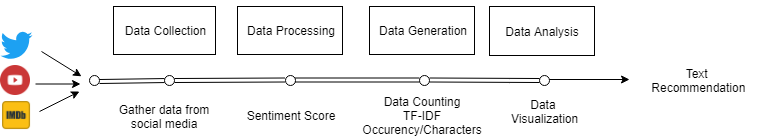
\includegraphics[width=0.8\linewidth]{img/Lexicon.png}
\end{center}
   \caption{Proposed approach overview: from data gathering to text recommendation.}
\label{fig:approach}
\end{figure*} 

The public opinion is one of the key factors for the success of a movie. To analyze and identify public opinion, we developed a sentiment analysis tool that, using tweets and comments from YouTube trailers, provides the following: \textit{i} The general public opinion about a movie; \textit{ii} The identification of the main topics on the evaluated texts; and \textit{iii} A ''recommendation text'' for the movie, based on the most relevant mentioned words. Next subsections describe all phases of the development to reach the proposed goal.

\subsection{Methodology}
\label{sec:Methodology}

Figure~\ref{fig:approach} presents our research methodology which is divided into five steps. The first one consists of collecting data from social media. On this step, we gathered data from both YouTube and Twitter, using the tools described in Subsection~\ref{sec:DataCollection}. Along with the scripts, this section details the data collection process as a whole.

After the Data Collection step, we executed the Data Processing step. During this second step, we used Vader to perform Sentiment Analysis on our texts.  This analysis provides us the sentiment scores and compound values for the tweets and comments collected. This step is fully detailed on Section \ref{sec:DataProcessing}
% I: não daria para complementar acima? Se eu entendi corretamentamente, no final do parágrafo acima poderia ter algo: Thus, we generate five files with the following content: (1) very positive; (2) positive; (3) neutral; (4) negative; and (5) very negative tweets and YouTube comments.
% Seria isto?



The fourth step of our study is the Data Analysis. On this step, we used the data generated data on the previous step to generate visualization charts. The goal of the visualization charts is to provide us information and statistics like the most frequent terms, the total of interaction, and others. Three visualization charts were generated on this step: a bar chart with the overall number of comments obtained, a word clouds presenting the most frequent words, and a heatmap showing the top 10 most used adjectives in movies comments. All these .visualizations are detailed described in Section \ref{sec:DataAnalysis}.


\subsection{Data Collection}
\label{sec:DataCollection}

For the context of movie reviews, we decided to analyze data from Twitter and YouTube comments about trailers. Twitter is used to quickly express opinions, and YouTube is a social media widely adopted to display movie trailers. We developed and used Python scripts to gather the desired data from the officials APIs of these social media. 

Twitter usually contain hashtags to indicate the subject of a text. Due to this reason, we chose to collect data through the use of hashtags instead of using keywords. We believe that the use of hashtags would provide a higher number of information and better quality data. The Twitter API implements features that allow a  user to provide a hashtag list with the subjects to be collected. Thus for each movie, we selected a different set of hashtags to be collected. 

The YouTube comments were collected from the Studios' officials channels. We collected data from all the officials' trailers released for a movie. In this analysis, we did not collect data from teasers. We only collect data from the top level of comments on YouTube. This decision was made because on the lower levels, the comments, generally, serve as an answer to previous comments and are not properly related to the movie. 

% I: estou em dúvida se o parágrafo abaixo não deveria ser o segundo parágrafo desta subseção. A ideia seria primeiro dizer como funcionam os scripts e depois explicar como foram feitas as coletas no contexto deste trabalho. Por exemplo, no Twitter foram usadas hashtags, e para o YouTube foram escolhidos os trailers oficiais dos studios. Trouxe para cá um texto que estava mais abaixo, e deixei os próximos dois parágrafos só com a descrição do que é coletado de cada rede social. Vejam se concordam com as alterações.
Both of our scripts are straight forward to use. The Twitter script just requires a list of hashtags to be collected and the YouTube script only requires the video ID. The video ID is easily spotted on its web address. The data collected from both scripts are stored on JSON files. The scripts used for data collection, along with a detailed description of how to use them, can be found on https://github.com/DAVINTLAB/TweetProcessing.

From Twitter, we collected data such as: \textit{username}, an internal user identification; \textit{lang}, the language in which the tweet was written; \textit{screen\_name}, user's name showed on screen; \textit{text}, the tweet written text; \textit{created\_at}, the date when the tweet was created; \textit{userid}, internal user identification; \textit{timezone}, the time zone in which the tweet was written; \textit{retweet\_count}, the number of times the tweet was re-posted; \textit{ID}, internal tweet identification; \textit{favorite\_count}, number of times other users liked this tweet.

From YouTube script, we collected the following data: \textit{publishedAt}, the date when the comment was posted; \textit{textOriginal}, the original comment text; \textit{likeCount}, the number of times another users liked the comment; and \textit{authorDisplayName}, the author name that is displayed on the screen. 

Besides the Twitter and YouTube scripts, we also developed a third script for the IMDB site. The main goal of this script is to provide a list of all the characters of a movie. Since the IMDB website does not provide an official API for this purpose, we used the free IMDBPY. API\footnote{https://imdbpy.sourceforge.io/}.

\subsection{Data Processing}
\label{sec:DataProcessing}

Sentiment analysis, also known as opinion mining, is a sub-field of Natural Language Processing (NLP)\cite{Indurkhya:2010}. The main purpose of Sentiment Analysis is to identify and extract impressions/opinions from a particular text~\cite{vader}. Although many improvements have already been done regarding the sentiment analysis area, this area still has opportunities for further enhancements, and so, there are several researches being developed for this area\cite{DEVIKA201644}.

Machine Learning is a widely used approach, and work by training an algorithm with a training data set, before applying it to the real data set\cite{DEVIKA201644}. This technique, first train the algorithm with some initials inputs, with known outputs, so that later it can work with new data\cite{He:2012}.

Lexicon based techniques work on the assumption that the collective polarity of a sentence or documents is the sum of polarities of individual phrases or words\cite{DEVIKA201644}. The term polarity lexicon is used to refer a dictionary or a vocabulary with the indications of positive and negative words with an associated score~\cite{Dipanjan:2016}. The difference between both approaches, is that the lexicon based does not need labeled data for testing\cite{DEVIKA201644}. 

% Classification techniques are based on word position, surrounding words, context analysis, part-of-speech, phrases, and others. 
Various lexicons may be used for this analysis. Examples are: AFINN Lexicon~\cite{afinn}\cite{anew}, Bing Liu's Lexicon~\cite{Jinda}, MPQA subjectivity Lexicon~\cite{Wilson}, SentiWordNet~\cite{esuli-sentiwordnet}\cite{baccianella-sentiwordnet}, Vader Lexicon~\cite{vader}, Pattern Lexicon~\cite{pattern}. 

In our research, we used Vader (Valence Aware Dictionary and sEntiment Reasoner)\footnote{https://github.com/cjhutto/vaderSentiment}
Lexicon to classify the tweets and comments from Youtube. In this approach, each word is labeled according to their semantic orientation as either positive or negative. Vader produces 4 sentiments metrics: the first three (positive, negative and neutral) represent the proportion of the words that match the categories. The final metric, \textit{compound} score, is a combination of the first three metrics normalized.
%SO normalizadas como?
The compound score ranges between -1 and 1, where -1 represents highly negative opinion and 1 highly positive opinion.

Since Vader deals with certain features that most of other lexicon do not (such as Abbreviations, Upper Case, Emojis, and Special characters), it is considered a very appropriate lexicon to be used in Social Media texts evaluation\cite{vader}. 
Through the example shown in Figure \ref{fig:tweet1}, we demonstrate the advantages of using Vader lexicon in Social Media.

%We consider using Vader Lexicon, to evaluate the tweets texts, for supporting the following aspects that non-normalized text may contain: Abbreviations, Upper Case, Emojis, Special characters. To understand, how Vader is great alternative to text analysis, follow a example: 

\begin{figure}[htb]
    \begin{center}
        
\includegraphics[width=0.8\linewidth]{img/Twitter1.png}
    \end{center}
       \caption{Example of a tweet post} %using Vader Lexicon.}
    \label{fig:tweet1}
\end{figure}

% I: acho que "tweet" já apareceu antes e não estava em itálico. Acho que não precisa colocar Tweet e Twitter em itálico. Revisar isso em todo o paper.
The tweet presented in Figure~\ref{fig:tweet1} was evaluated with the following scores for sentiment analysis: \textit{'compound'}: 0.6133, \textit{'neg'}: 0.169, \textit{'neu'}: 0.508, \textit{'pos'}: 0.322. As we can see, the overall evaluation of the text denotes a positive emotion. But if this same text was parsed without considering \textit{emojis} and the emotional indication represented by capital letters, 
%SO: mudei um pouco a frase acima para explicar o "capital letters".. mas na verdade não entendi esse parágrafo, fiquei com muitas duvidas. Joana, podes passar aqui?
the scores evaluation would be: \textit{'compound'}: 0.2043, \textit{'neg'}: 0.202, \textit{'neu'}: 0.546, \textit{'pos'}: 0.251. In this case, we can notice a significant drop on the \textit{compound} value, which makes the text's emotion tending to neutral, instead of positive.% as it should.
%SO: tens que explicar o que são esses parametros? compound indica o que?


\subsection{Dataset Generation}
\label{sec:DataGeneration}

\textit{Term Frequency-Inverse Document Frequency} indicates the weight of text's terms according to its frequency proportion~\cite{Dipanjan:2016} across documents. This is a well-known metric in information retrieval, and help us to identify the most recurrent terms in texts, allowing us to create visualization that work essentially with the use of words.

\begin{equation*}
    W_{t,d} = \left ( \frac{Freq_{t,d}}{Max} \right ) * log_2 \left ( \frac{N}{n_t} \right),
\end{equation*}
where \( W_{t,d}\) represents the term weight \textit{t} in document \textit{d}. 
\( Freq_{t,d}\) is the number of times that the terms ($t$) occurrences in document \textit{d}. 
\( Max\) is the total number of all words in document. 
\( N \) is how many times the term appears, \( n_t \) is number of documents containing the term \( t \). Applying the TF-IDF calculation, on the set of texts classified by Vader, we generate 5 outputs files, according to their polarity and with the structure as shown in the Listing \ref{tfidf}.

\begin{lstlisting}[label=tfidf,caption=TF-IDF File Structure,float,frame=tb]
    [('ragnarok', 'NN')],256
    [('saying', 'VBG')],2152
    [('rich', 'JJ')],125
    [('lots', 'NNS')],102
    [('much', 'JJ')],3509
\end{lstlisting}


%To understand how the public reacted to each character, it's necessary to have knowledge about the occurrences of the most used terms in relation to the main characters of a movie. This process is composed of 4 phases, as shown in Figure~\ref{fig:phases}. 
To understand how the public reacted to each character, it's necessary to know the number of occurrences of most used terms for each character. This process is consists of 4 phases, as shown in Figure~\ref{fig:phases}. 

For the first phase, we needed the list characters from the movie. So, we used the characters list generated by the IMDB script described in Section \ref{sec:DataCollection}. Then, for each character on
the list, we searched the set of texts classified by Vader % pelo q?
and store the texts that have this condition in a temporary list. On the third phase, we tried to find in the resulting TF-IDF files, the terms classified as adjectives which had at least 100 occurrences in texts. This result is also saved in a temporary list.  

%The last phase, is concerned with run the temporary list of text generated in phase 2, in the search for terms established in the phase 3. If condition is true, we add in a incremental variable, the number of times a given term is mentioned for each character, generating a occurrence file (Figure \ref{fig:occurs}). 
The last phase consists in %aqui
run the temporary list of text generated in phase 2, in the search for terms established in the phase 3. If condition is true, we add in a incremental variable, the number of times a given term is mentioned for each character, generating a occurrence file (Figure \ref{fig:occurs}). 

% 1 - lista de personagens
% 2 - textos classificados pelo vader, verifica se encontra os personagens da lista, se encontrar coloca em uma lista temporaria
% 3 - files tf-idf e busca so os adjetivos e guarda em lista temporaria 

\begin{figure}[h]
    \begin{center}
        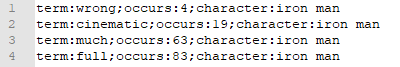
\includegraphics[width=0.8\linewidth]{img/occurs.png}
    \end{center}
       \caption{Occurrence File.} 
    \label{fig:occurs}
\end{figure}

\begin{figure*}[btp]
\begin{center}
% \fbox{\rule{0pt}{2in} \rule{.9\linewidth}{0pt}}
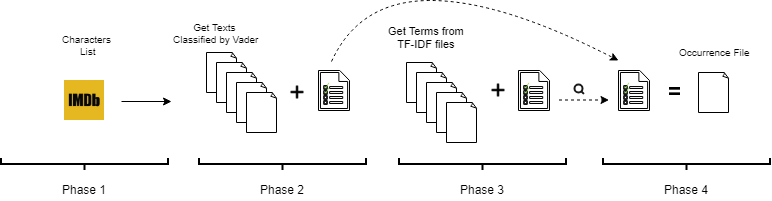
\includegraphics[width=0.8\linewidth]{img/diagrama-ocorrencia-movie.png}
\end{center}
   \caption{Occurrence Terms Model.}
\label{fig:phases}
\end{figure*}

\subsection{Data Analysis}
\label{sec:DataAnalysis}

For this paper, as mention before, we generated 3 visualization graphics for each social media we chose. The first one is a bar chart that displays the overall number of comments obtained for the selected movies on both social media. Each bar presented on this visualization represents one sentiment polarity (very positive, positive, negative and very negative). We opted to display the social media side by side to simplify users' comparison. 

The second visualization provides word clouds, showing the most used words for negative and positive sentiment polarity. For this visualization, we chose to use only verbs, noun, and adjective grammar types, because, for this case, we believe that those are the most significant ones. Like the previous visualization, 2 word clouds are generated for each social media, one for the most used words in negative comments, and another one for the most used words in positive comments. 

On the third visualization, a heatmap is presented. This visualization presents the top 10 most used adjectives in comments for the movie's characters. For this visualization, we present only characters for whom we were able to find mentions in the analyzed text. This visualization is split by sentiment polarity (positive and negative) and by social media (Twitter and YouTube). These visualizations can be seen in Figures ~\ref{fig:TotalOfInteractions},~\ref{fig:wordcloudsAquaman},~\ref{fig:wordcloudsCaptain},~\ref{fig:wordcloudsAvengers},~\ref{fig:AquamanCapitaHeatMap} and \ref{fig:VingadoresHeatMap}.

\subsection{Text Recomendation}
\label{sec:TextualRecomendation}





%\section{Data Analysis}



\section{RESULTS AND DISCUSSION}
\label{sec:results}
%Uso da abordagem nos três estudos de dados (Avengers, Aquaman, Capitã Marvel), análise dos resultados e contribuições.

\begin{figure*}[htb]
\begin{center}
% \fbox{\rule{0pt}{2in} \rule{.9\linewidth}{0pt}}
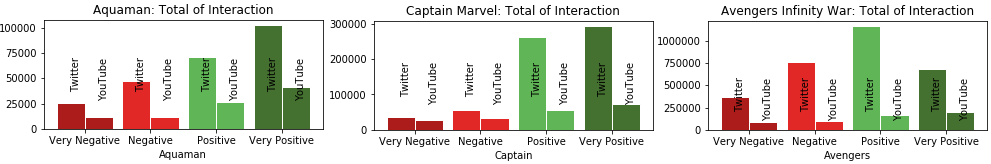
\includegraphics[width=1.0\linewidth]{img/TotalInteractions2.png}
\end{center}
   \caption{Total number of interactions for each movie.}
   % I: acima é preciso especificar porque tem duas barras. Por exemplo: The first bar in each polarity represents the interactions on Twitter and the second on YouTube. 
\label{fig:TotalOfInteractions}
\end{figure*}

%JS: Revisado com o pedro
For the purpose of demonstrating the applicability of our visual analysis approach, we selected three case-studies regarding recently released blockbuster movies to be detailed in the following subsections. We chose these movies in consideration of their popularity in social media, which generated a large volume of data to be analyzed.

\subsection{Dataset Description}

%JS: Mudei o paragrafo abaixo, pois ficou meio repetitivo com o de cima.

%original
%To evaluate the developed approach, we collected data from three major movies releases of the years 2018 and 2019: Avengers Infinite War\footnote{https://www.marvel.com/movies/avengers-infinity-war}, Aquaman\footnote{http://www.aquamanmovie.net/}, and Captain Marvel\footnote{https://www.marvel.com/movies/captain-marvel}. The data gathering process occurred during the debut week of each movie, as showed in Table~\ref{tab:range_data}. 

Our case study data was collected from three major movies releases of the years 2018 and 2019: Avengers Infinite War~\footnote{https://www.marvel.com/movies/avengers-infinity-war}, Aquaman~\footnote{http://www.aquamanmovie.net/}, and Captain Marvel~\footnote{https://www.marvel.com/movies/captain-marvel}. For Twitter, the data gathering process occurred during the debut week of each movie, as showed in Table~\ref{tab:range_data}. For YouTube, we collected all comments available in the official trailers until 03/18/2019, which is the day when the script was executed. 

\begin{table}[h]
    \small{}
    \begin{tabular}{ p{4cm}|p{1.5cm}|p{1.5cm} }
        \hline
            \textbf{Movie} & \textbf{Start} & \textbf{Final}\\
        \hline
            Avengers Infinite War & 04/20/2018  & 05/04/2018 \\
            Aquaman & 12/03/2018 & 12/17/2018  \\
            Captain Marvel & 03/10/2019 & 03/18/2019 \\
        \hline
    \end{tabular}
    \caption{Range of  Twitter data collection.}
    % I: Alterei a legenda acima. A original era: Range of Data Collection. Vejam se concordam.
    \label{tab:range_data}
\end{table}


For data gathering, we used the tools described in Subsection~\ref{sec:datasetCollection}. For Twitter data collection, we used the hashtags: \#AvengersInfinityWar and \#InfinityWar for the Avengers Infinite War movie; \#Aquaman for the Aquaman movie; and \#CaptainMarvel for the Captain Marvel movie. For YouTube, the comments were collected through Marvel's and DC's official YouTube channel\footnote{Infinity War: https://www.youtube.com/watch?v=6ZfuNTqbHE8 and https://www.youtube.com/watch?v=QwievZ1Tx-8}\footnote{Aquaman: https://www.youtube.com/watch?v=WDkg3h8PCVU and https://www.youtube.com/watch?v=fKnL0005qEU}\footnote{Captain Marvel: https://www.youtube.com/watch?v=Z1BCujX3pw8 and https://www.youtube.com/watch?v=0LHxvxdRnYc}.

Our final dataset was distributed as follows: 2.985.563 tweets and 553.618 YouTube comments for Avengers Infinite War; 246.344 tweets and 91.634 YouTube comments for Aquaman; and 650.730 tweets and 189.972 YouTube comments for Captain Marvel. 



\subsection{Results Analysis}

% I: reescrevi o parágrafo abaixo, original em comentário.
The first visualization developed was the bar chart presented in Figure \ref{fig:TotalOfInteractions}. This chart provides an overview of the total and the polarity of tweets in each dataset. It is possible to notice that the Avengers movie was, by far, the most commented movie from the selected 3. It is also possible to see that, even though the collection period is longer on YouTube, most comments were made on Twitter.

Another aspect that can be noticed on this chart is that the proportion between the number of comments in each polarity does not remain the same on YouTube and Twitter. For instance, the number of very negative and negative comments on YouTube remains almost the same for all analyzed movies, but there are significant differences for it on Twitter.
% I: não sei se dá para fazer a afirmação acima... Teria que ver em percentual, não em número absoluto. Mas, deixa isso para o final, só se der tempo.

% I: abaixo não faltou especificar para qual filme no primeiro aspecto? Não seria: The first one was that the number of positive comments overcomes the number of very positives just for Avengers.?
Two other aspects of these charts surprised us. The first one was that the number of positive comments overcomes the number of very positives. The second one was that Captain Marvel had the least amount of negative comments from the overall group. 
The second visualization we developed was the word clouds presented in the Figures~\ref{fig:wordcloudsAquaman}, \ref{fig:wordcloudsCaptain} and \ref{fig:wordcloudsAvengers}. These word clouds provided some meaningful insights about our data. For instance, we can have an idea of which characters will appear on the heatmaps chart. In the word cloud of the movie Avengers, it is possible to notice that the character ''Thanos'' appears on both positive and negative word clouds, and checking the heatmaps, we can verify that he is one of the most mentioned ones.
% I: alterei um pouco o final do parágrafo acima. Original abaixo. Mas, na fig. 6, eu não vi o Thanos nas word clouds positivas, pelo menos não tão grande como nas negativas. Ou estou enganada? Então não seria o caso de dizer que ele aparece nas negativas por ser o vilão da história?
%It is possible to notice that the character ``Thanos'' appears on both positive and negative word clouds, checking the heatmaps, we can verify that he is one of the most mentioned ones.

% I: uma curiosidade é porque o Thanos aparece nas word cloud negativa da capitã Marvel? Talvez possa se dizer que são feitas comparações entre eles, de quem é o mais poderoso. Mas, para isso, teria que pegar alguns tweets de exemplo para justificar a afirmação. Outra curiosidade é porque aparece "panther" na word cloud do filme do Aquaman, se eles são de universo diferentes? De novo, teria que pegar tweets que tenham panther para ver o que dizem...

% I: o que é CGI abaixo? Esta sigla não foi usada antes.
Also, the majority of words used to generate the ``recommendation text'' can be seen in the word clouds. For instance, words like good and best can be seen on the positive word clouds for the Avengers movie, and CGI (computer-generated imagery) can be seen on the negative YouTube word cloud for Aquaman.

Analyzing the word clouds as a whole, we can notice several differences between the Twitter version and the YouTube one. The YouTube word clouds focus more on expectation and technical aspects of the movie, while the Twitter one focus more on viewers' opinions.

% I: abaixo já é sobre o heat map? É que o parágrafo está começando de forma genérica  (The visualization we provided...).
The visualization we provided, shows which ones are the most commented characters of a movie, and the most common words used to describe it. In the same way as the word cloud visualization, we can notice that the words used in YouTube are different from the ones used on Twitter. Regarding the characters, they remain relatively the same on both social media, with some minor differences.

Also, for the characters is possible to notice that, if a character has a high number of interaction in one social media, it is most likely to have a high number of communications on the other ones. This statement is also valid for the heatmap polarity. If a character was highly commended in the positive heatmap, it probably will, also, appear on the negative heatmap. There are a few exceptions for this statement like, for instance, the Black Widow character on Twitter and Korath character on YouTube.

\begin{figure*}[htb]
\begin{center}
    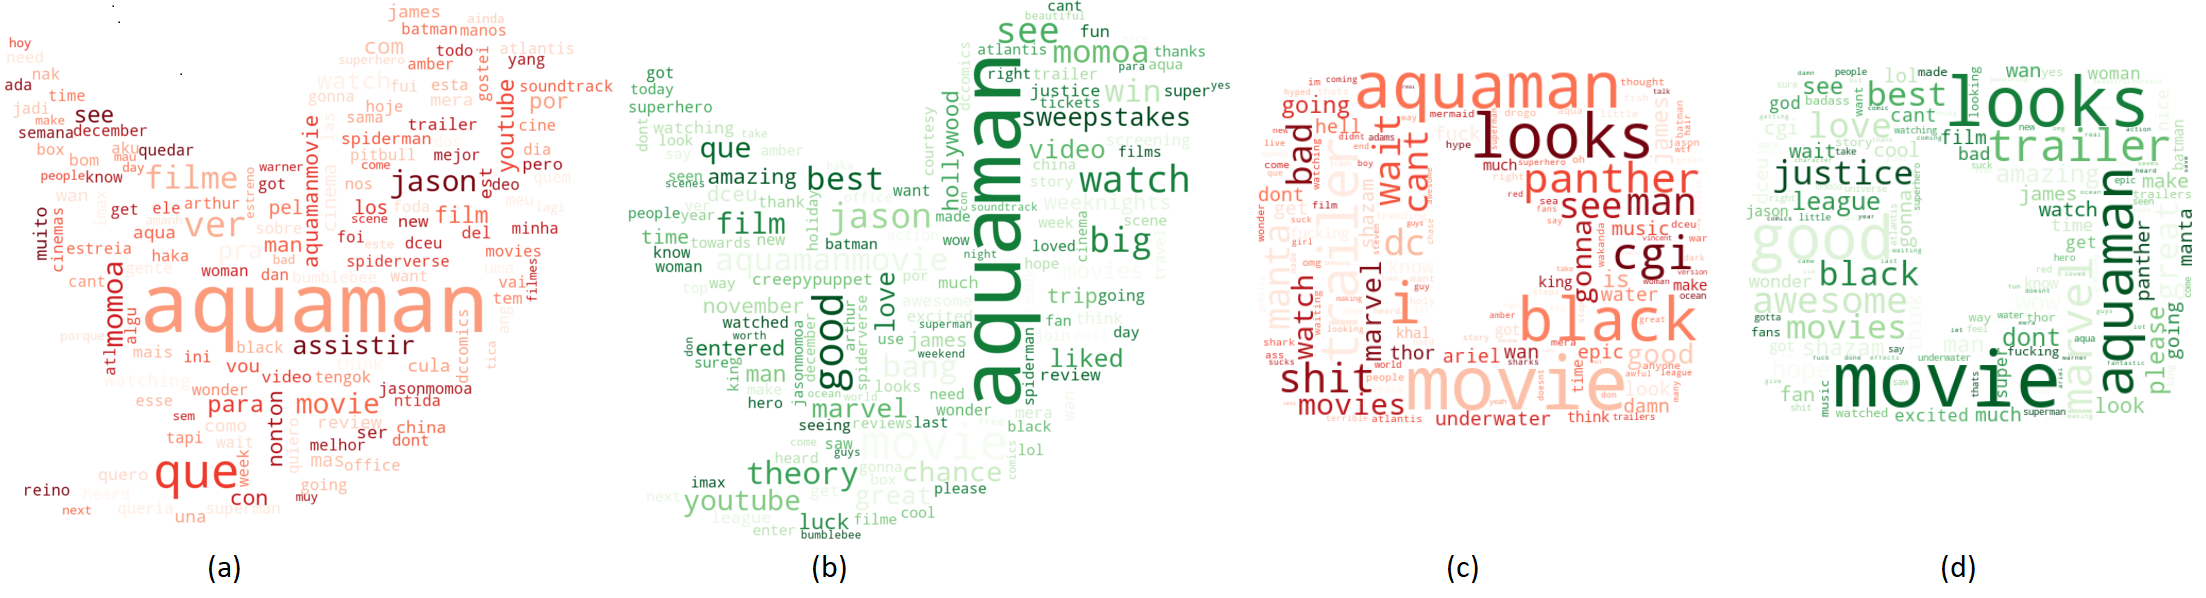
\includegraphics[width=1\linewidth]{img/wordcloudsAquaman.png}
\end{center}
  \caption{Positive (green) and negative (red) word clouds with most used terms in Tweets (a,b) and YouTube comments (b,c) about Aquaman movie.}
  % I: quem sabe alterar a legenda acima para:
  % Positive (green) and negative (red) word cloud with most used terms in Tweets (a,b) and YouTube comments (b,c) about Aquaman movie.
  % Se concordarem, usar o mesmo "padrão" nas demais. 
\label{fig:wordcloudsAquaman}
\end{figure*}

\begin{figure*}[htb]
\begin{center}
    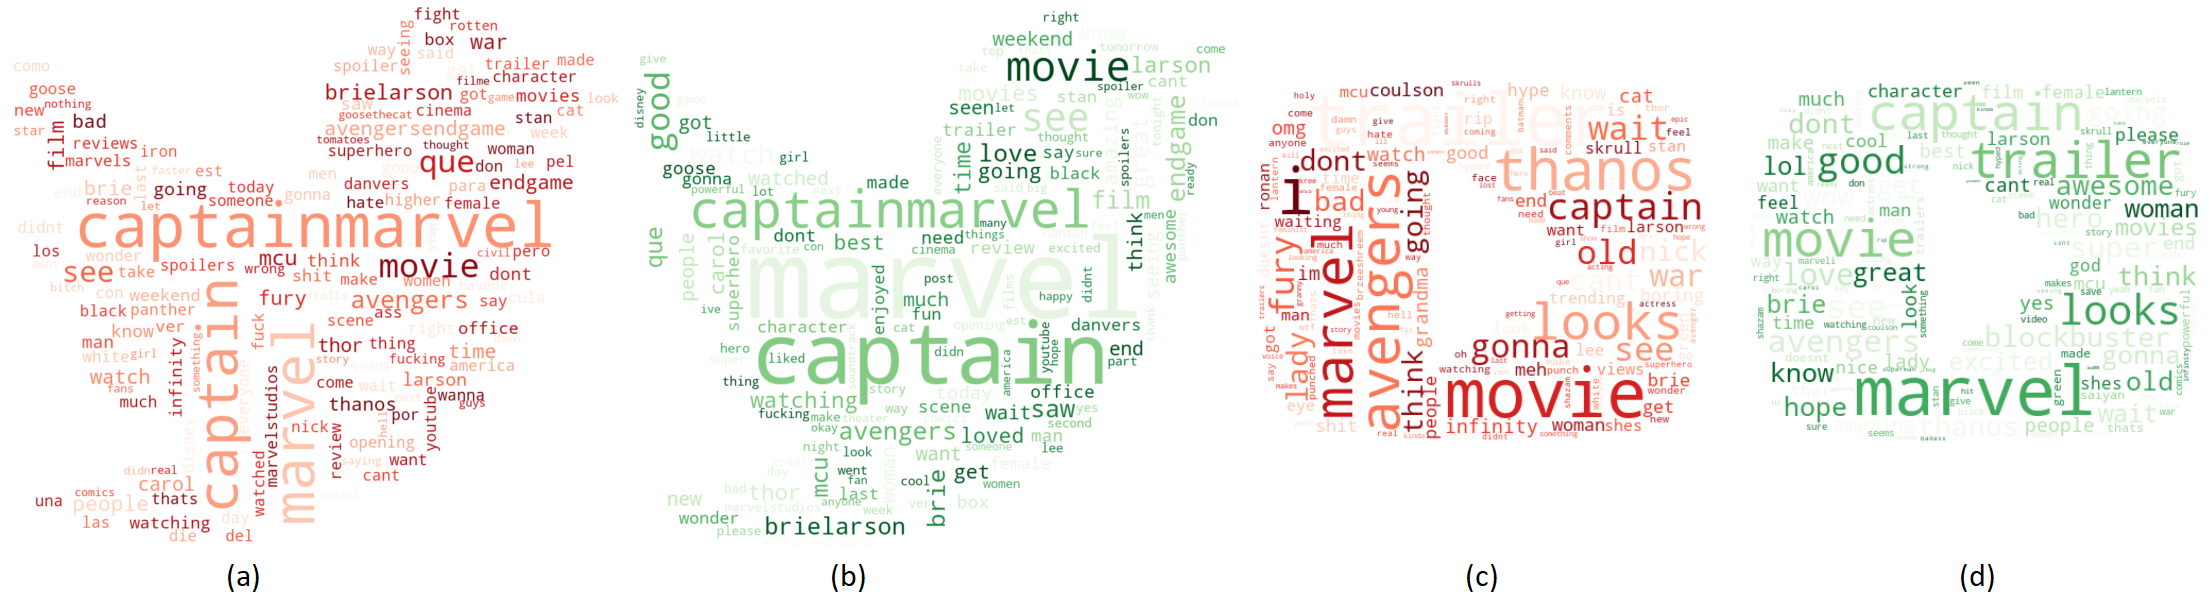
\includegraphics[width=1\linewidth]{img/wordcloudsCaptain.png}
\end{center}
  \caption{Positive (green) and negative (red) word clouds with most used terms in Tweets (a,b) and YouTube comments (b,c) about Captain Marvel movie.}
\label{fig:wordcloudsCaptain}
\end{figure*}

\begin{figure*}[htb]
\begin{center}
    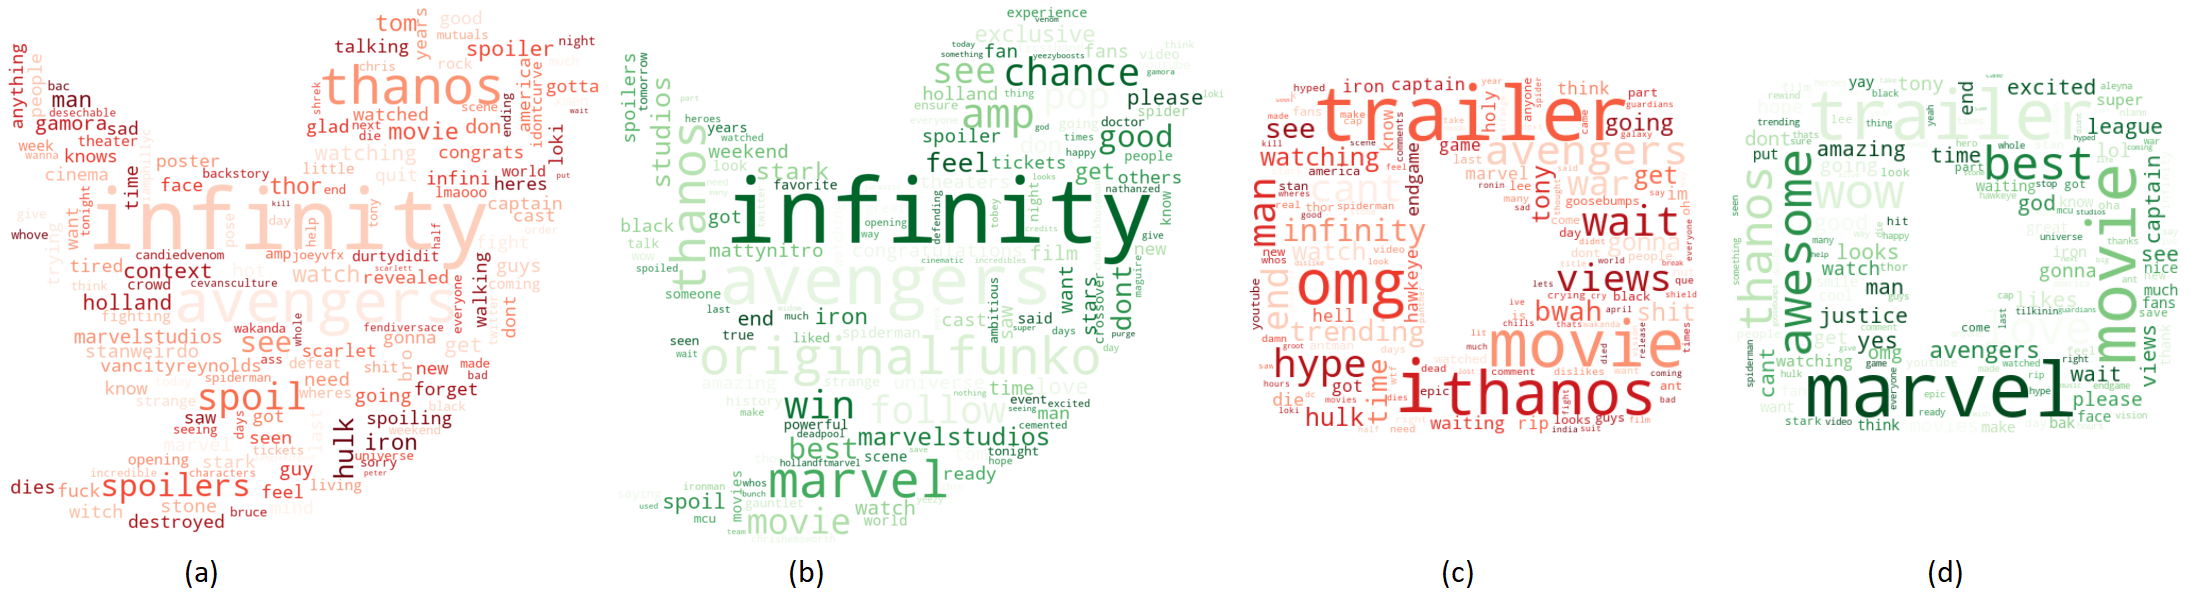
\includegraphics[width=1\linewidth]{img/wordcloudsAvengers.png}
\end{center}
  \caption{Positive (green) and negative (red) word clouds with most used terms in Tweets (a,b) and YouTube comments (b,c) about Avengers Infinity War movie.}
\label{fig:wordcloudsAvengers}
\end{figure*}

%
\begin{figure*}[htb]
\begin{center}
    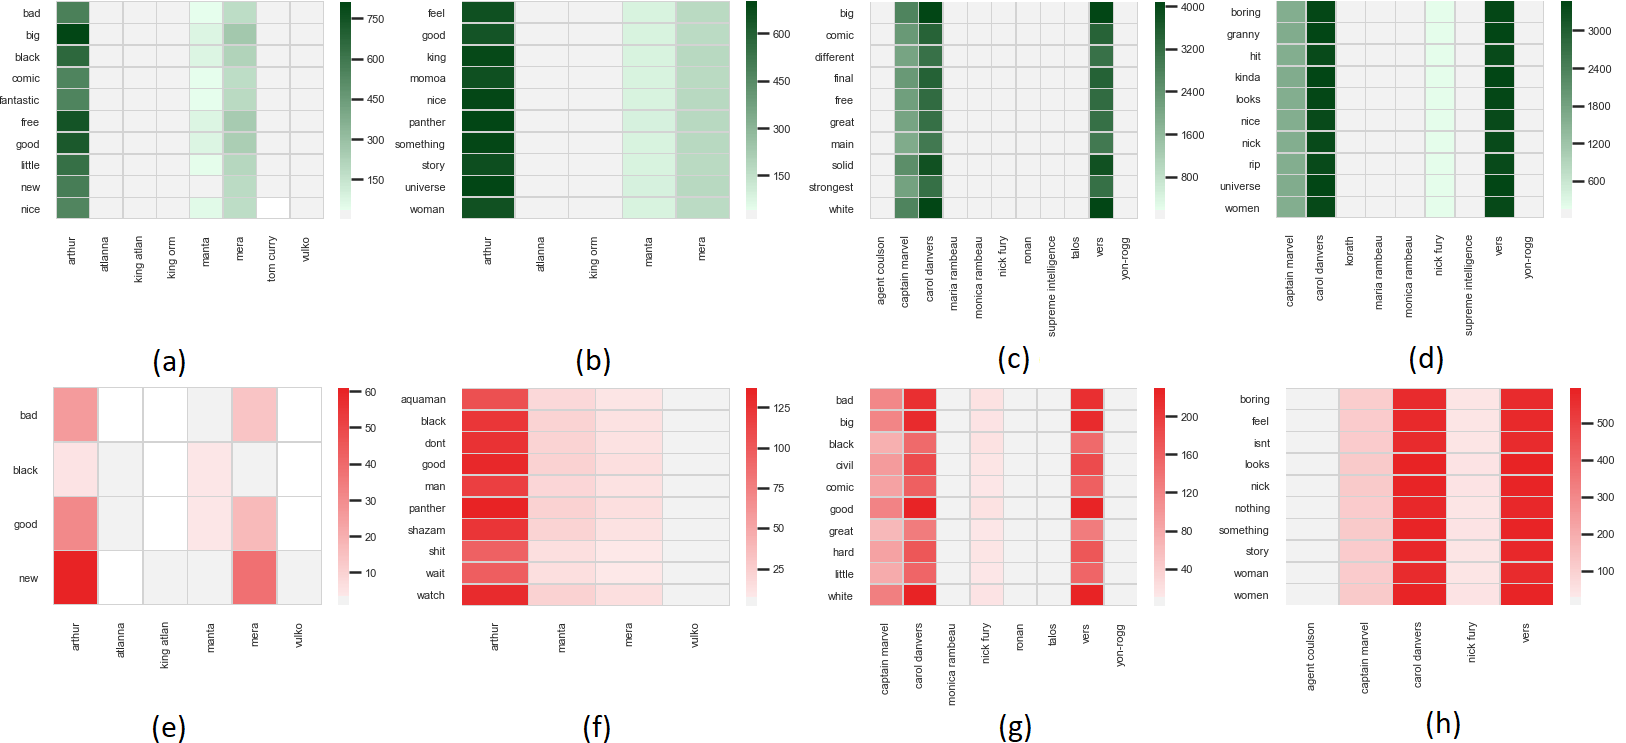
\includegraphics[width=1\linewidth]{img/AquamanCapitaHeatMap.png}
\end{center}
   \caption{Positive (green) and negative (red) heatmaps with the top 10 most used words to describe character in Tweets and YouTube comments. Twitter positive heatmap for Aquaman (a); YouTube positive heatmap for Aquaman (b); Twitter positive heatmap for Captain Marvel (c); YouTube positive heatmap for Captain Marvel (d);
   Twitter negative heatmap for Aquaman (e); YouTube negative heatmap for Aquaman (f); Twitter negative heatmap for Captain Marvel (g). YouTube negative heatmap for Captain Marvel (h).}
   % I: Quando arrumar esta legenda, especificar cada letra.
\label{fig:AquamanCapitaHeatMap}
\end{figure*}

\begin{figure*}[htb]
\begin{center}
    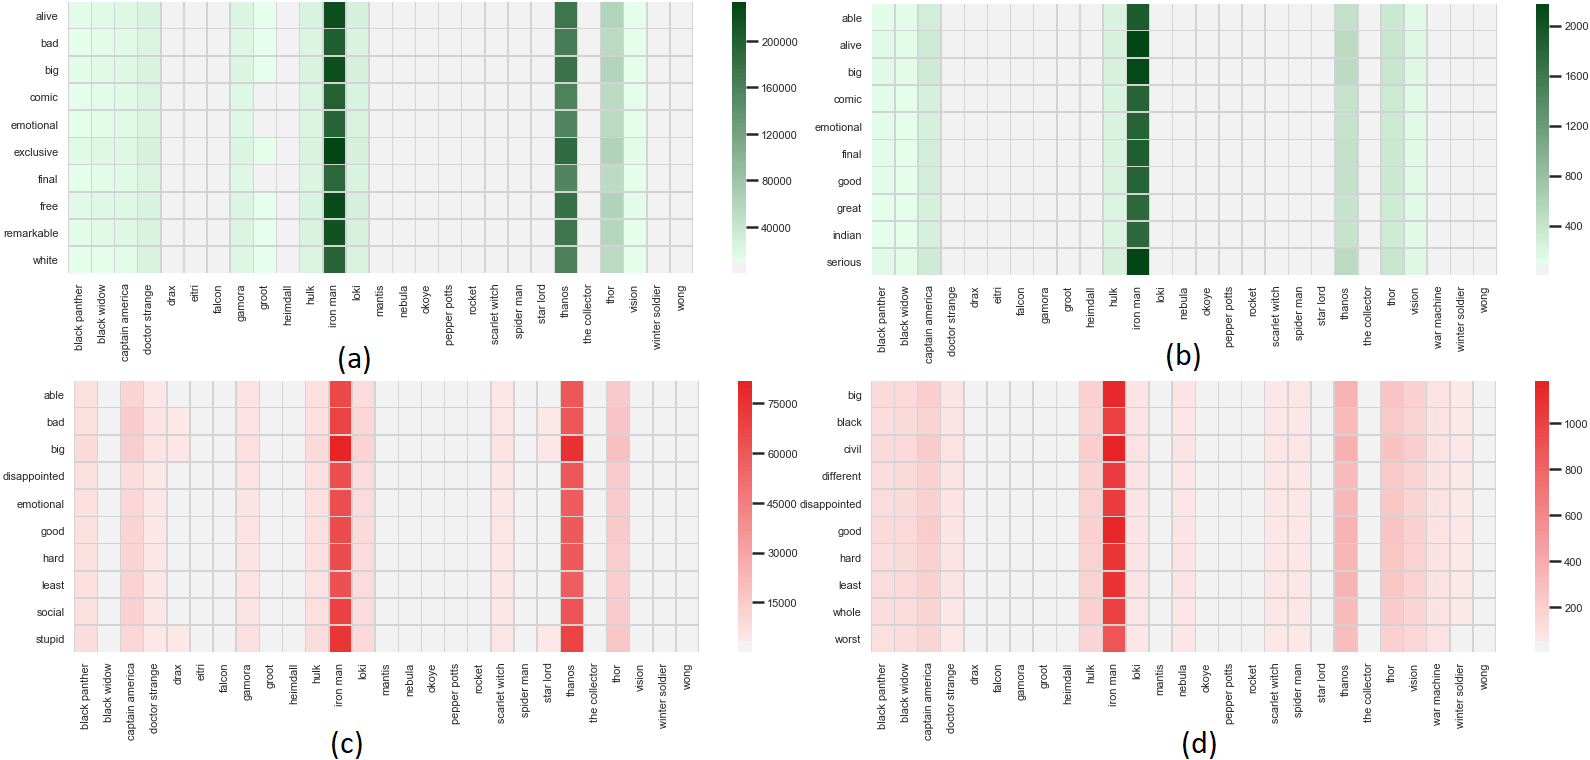
\includegraphics[width=1\linewidth]{img/VingadoresHeatMap.png}
\end{center}
   \caption{Positive (green) and negative (red) heatmaps with the top 10 most used words to describe character in Tweets and YouTube comments. Twitter positive heatmap (a); YouTube positive heatmap (b); Twitter positive heatmap (c); YouTube positive heatmap (d) for Avengers Infinity War.}
\label{fig:VingadoresHeatMap}
\end{figure*}

\subsection{Textual recommendation and Word Clouds}

%In this step, we use the TF-IDF features to evaluate how important is a certain term/word in a given document~\cite{Dipanjan:2016}. From the results obtained by the lexicons, we divided in files, according with texts polarity, to calculate the TF-IDF. Therefore, we will have the most used terms in negative and positive texts.

% In this step, we use the TF-IDF features to evaluate how important a certain term/word is in a given document~\cite{Dipanjan:2016}. The results obtained by the sentiment analysis with Vader, were divided into files, according to the polarity defined by the lexicon in each text, and then the TF-IDF was applied. Therefore, we will have the most used terms in negative and positive texts.

%In this step, we used TF-IDF features to evaluate how important a certain term/word is in a given document. The results obtained by the lexicons were divided into files, according to their polarity, and then the TF-IDF was applied. Therefore, we will have the most used terms in negative and positive texts. 
%SO: aqui acima... no passo a passo ainda não sabemos se é positivo ou neg no paragrafo acima né? achei essa section mal explicada e confusa

% From the most used terms found in the texts, we proceed to the identification the lexical category in which the words are assigned based on their syntactic context and role, called POS (Part-of-Speech) Tagging. Using NLTK Library, which generates outputs specific tags for certain word, we could find: \textit{Adjectives, Nouns, Adverbs, Coordination Conjunction, Verbs, Preposition and etc}, as showed in Listing \ref{tfidf}. 

%SO: ao invés deste "can mention", que tal "could find"



Manually, we created text recommendations about analyzed movies, based on the terms generated by TF-IDF, respecting the text's syntatic structure. The Text Recommendation is presented in Table~\ref{ref:text-rec}.  

\begin{table}[h!]    
    \small
    \begin{tabular}{  l | p{6cm} }
    \hline
        \textbf{Movie} & \textbf{Text Recommendation} \\ 
    \hline
        \multirow{6}{*}{\textbf{Avengers}} & \textbf{Pos:} Avengers was \textit{greatest, biggest, best} movie I had seen. With \textit{huge} and \textit{fantastic} fight scenes, and \textit{hilarious} dialogues between the characters. \textbf{Neg:} Avengers made me \textit{angry, depressed, worried, and physically weak} with the final scene. \\ 
    \hline
        \multirow{6}{*}{\textbf{Aquaman}} & \textbf{Pos:} Aquaman \textit{impressed} (\textit{surprised}) me \textit{positively}, with \textit{incredibles} visual effects. DC Comics has built a great, fantastic and solid movie for all fans. \textbf{Neg:} Aquaman has \textit{missing cgi} in some scenes, in addition to \textit{exploring} little \textit{fight} scenes. \\ 
    \hline
        \multirow{8}{*}{\textbf{Captain M.}} & \textbf{Pos:} Captain Marvel proved \textit{strong, powerful} and \textit{ready} for any battle. Marvel delivered an \textit{important character}, capable of impressing the \textit{capable impressing audience} that didn't know it. \textbf{Neg:} The movie \textit{reminds} me \textit{Green Lantern}. And the way she got your \textit{powers}, wasn't well \textit{solved} in the movie.\\
    \hline
    \end{tabular}
    \caption{Text Recommendation about movies.}
    \label{ref:text-rec}
\end{table}

In addition, we present Word Clouds based on results from TF-IDF. The corpus of these Word Clouds is about texts extracted from tweets during week premiere, and trailers comments on YouTube. It contains all the main terms, organized by color, red for negative and very negative terms, green for positive and very positive, by mask according to the social network, and by movie, as shown in Figures \ref{fig:wordcloudsAquaman}, \ref{fig:wordcloudsCaptain}, \ref{fig:wordcloudsAvengers}.

% \subsection{HeatMap}

% The Heat Map build, aims to show the degree most used terms occurrences in relation to the main characters of each movie. This process is composed of 4 phases. The first phase, is to collect the list of main characters in each movie. Then, we search for each character in the list, in the set of already classified texts, and store the texts that have this condition in a temporary list. 

% The third phase, we try to find in the resulting TF-IDF files, the terms classified as \textit{Adjectives} and that have at least 100 appearances in texts, and we also save in a temporary list. The last phase, is concerned with run the temporary list of text generated in phase 2, in the search for terms established in the phase 3. If condition is true, we add in a incremental variable, the number of times a given term is mentioned for each character. 

%SO: acima nos resultados... aquele texto a direita pe de alguem especifico? ou gerado?



\section{CONCLUSIONS AND FUTURE WORK}
\label{sec:conclusions}

We present a new approach for the visual analysis of viewers comments on two social media: Twitter and YouTube. It analyzes and synthesizes the public opinion concerning a movie, highlighting what are being discussed and the public satisfaction in those platforms. We showed the obtained results through three case studies where we analyze three blockbuster movies, displaying public opinion before and after its release.

Our contribution is mainly the generation of a ``recommendation text'' through the application of an unsupervised lexicon-based approach, which represents the public opinion about a certain movie.  Another contribution is that our approach allows a visual analysis of the collected data showing the total number of interaction, the most frequent terms, and the adjective used for the main characters. 

% I: "inventei" uma atividade para dizer que estamos fazendo "agora"... 
We are now working in the implementation of an interactive interface to facilitate the visual analysis. For our future works, we intend to analyze the use of \textit{Dirty Words}, to identify if there is an intensification of the sentiment expressed in previous classification. 



%\subsection{Selecting a Template (Heading 2)}

%First, confirm that you have the correct template for your paper size. This template has been tailored for output on the US-letter paper size. Please do not use it for A4 paper since the margin requirements for A4 papers may be different from Letter paper size.

%\subsection{Maintaining the Integrity of the Specifications}

%The template is used to format your paper and style the text. All margins, column widths, line spaces, and text fonts are prescribed; please do not alter them. You may note peculiarities. For example, the head margin in this template measures proportionately more than is customary. This measurement and others are deliberate, using specifications that anticipate your paper as one part of the entire proceedings, and not as an independent document. Please do not revise any of the current designations

%\section{MATH}

%Before you begin to format your paper, first write and save the content as a separate text file. Keep your text and graphic files separate until after the text has been formatted and styled. Do not use hard tabs, and limit use of hard returns to only one return at the end of a paragraph. Do not add any kind of pagination anywhere in the paper. Do not number text heads-the template will do that for you.

%Finally, complete content and organizational editing before formatting. Please take note of the following items when proofreading spelling and grammar:

%\subsection{Abbreviations and Acronyms} Define abbreviations and acronyms the first time they are used in the text, even after they have been defined in the abstract. Abbreviations such as IEEE, SI, MKS, CGS, sc, dc, and rms do not have to be defined. Do not use abbreviations in the title or heads unless they are unavoidable.

%\subsection{Units}

%\begin{itemize}

%\item Use either SI (MKS) or CGS as primary units. (SI units are encouraged.) English units may be used as secondary units (in parentheses). An exception would be the use of English units as identifiers in trade, such as Ò3.5-inch disk driveÓ.
%\item Avoid combining SI and CGS units, such as current in amperes and magnetic field in oersteds. This often leads to confusion because equations do not balance dimensionally. If you must use mixed units, clearly state the units for each quantity that you use in an equation.
%\item Do not mix complete spellings and abbreviations of units: ÒWb/m2Ó or Òwebers per square meterÓ, not Òwebers/m2Ó.  Spell out units when they appear in text: Ò. . . a few henriesÓ, not Ò. . . a few HÓ.
%\item Use a zero before decimal points: Ò0.25Ó, not Ò.25Ó. Use Òcm3Ó, not ÒccÓ. (bullet list)

%\end{itemize}


%\subsection{Equations}

%The equations are an exception to the prescribed specifications of this template. You will need to determine whether or not your equation should be typed using either the Times New Roman or the Symbol font (please no other font). To create multileveled equations, it may be necessary to treat the equation as a graphic and insert it into the text after your paper is styled. Number equations consecutively. Equation numbers, within parentheses, are to position flush right, as in (1), using a right tab stop. To make your equations more compact, you may use the solidus ( / ), the exp function, or appropriate exponents. Italicize Roman symbols for quantities and variables, but not Greek symbols. Use a long dash rather than a hyphen for a minus sign. Punctuate equations with commas or periods when they are part of a sentence, as in

%$$
%\alpha + \beta = \chi \eqno{(1)}
%$$

%Note that the equation is centered using a center tab stop. Be sure that the symbols in your equation have been defined before or immediately following the equation. Use Ò(1)Ó, not ÒEq. (1)Ó or Òequation (1)Ó, except at the beginning of a sentence: ÒEquation (1) is . . .Ó

%\subsection{Some Common Mistakes}
%\begin{itemize}


%\item The word ÒdataÓ is plural, not singular.
%\item The subscript for the permeability of vacuum ?0, and other common scientific constants, is zero %with subscript formatting, not a lowercase letter ÒoÓ.
%\item In American English, commas, semi-/colons, periods, question and exclamation marks are located within quotation marks only when a complete thought or name is cited, such as a title or full quotation. When quotation marks are used, instead of a bold or italic typeface, to highlight a word or phrase, punctuation should appear outside of the quotation marks. A parenthetical phrase or statement at the end of a sentence is punctuated outside of the closing parenthesis (like this). (A parenthetical sentence is punctuated within the parentheses.)
%\item A graph within a graph is an ÒinsetÓ, not an ÒinsertÓ. The word alternatively is preferred to the word ÒalternatelyÓ (unless you really mean something that alternates).
%\item Do not use the word ÒessentiallyÓ to mean ÒapproximatelyÓ or ÒeffectivelyÓ.
%\item In your paper title, if the words Òthat usesÓ can accurately replace the word ÒusingÓ, capitalize the ÒuÓ; if not, keep using lower-cased.
%\item Be aware of the different meanings of the homophones ÒaffectÓ and ÒeffectÓ, ÒcomplementÓ and ÒcomplimentÓ, ÒdiscreetÓ and ÒdiscreteÓ, ÒprincipalÓ and ÒprincipleÓ.
%\item Do not confuse ÒimplyÓ and ÒinferÓ.
%\item The prefix ÒnonÓ is not a word; it should be joined to the word it modifies, usually without a hyphen.
%\item There is no period after the ÒetÓ in the Latin abbreviation Òet al.Ó.
%\item The abbreviation Òi.e.Ó means Òthat isÓ, and the abbreviation Òe.g.Ó means Òfor exampleÓ.

%\end{itemize}


%\section{USING THE TEMPLATE}

%Use this sample document as your LaTeX source file to create your document. Save this file as {\bf root.tex}. You have to make sure to use the cls file that came with this distribution. If you use a different style file, you cannot expect to get required margins. Note also that when you are creating your out PDF file, the source file is only part of the equation. {\it Your \TeX\ $\rightarrow$ PDF filter determines the output file size. Even if you make all the specifications to output a letter file in the source - if you filter is set to produce A4, you will only get A4 output. }

%It is impossible to account for all possible situation, one would encounter using \TeX. If you are using multiple \TeX\ files you must make sure that the ``MAIN`` source file is called root.tex - this is particularly important if your conference is using PaperPlaza's built in \TeX\ to PDF conversion tool.

%\subsection{Headings, etc}

%Text heads organize the topics on a relational, hierarchical basis. For example, the paper title is the primary text head because all subsequent material relates and elaborates on this one topic. If there are two or more sub-topics, the next level head (uppercase Roman numerals) should be used and, conversely, if there are not at least two sub-topics, then no subheads should be introduced. Styles named ÒHeading 1Ó, ÒHeading 2Ó, ÒHeading 3Ó, and ÒHeading 4Ó are prescribed.

%\subsection{Figures and Tables}

%Positioning Figures and Tables: Place figures and tables at the top and bottom of columns. Avoid placing them in the middle of columns. Large figures and tables may span across both columns. Figure captions should be below the figures; table heads should appear above the tables. Insert figures and tables after they are cited in the text. Use the abbreviation ÒFig. 1Ó, even at the beginning of a sentence.

%\begin{table}[h]
%\caption{An Example of a Table}
%\label{table_example}
%\begin{center}
%\begin{tabular}{|c||c|}
%\hline
%One & Two\\
%\hline
%Three & Four\\
%\hline
%\end{tabular}
%\end{center}
%\end{table}


%  \begin{figure}[thpb]
%      \centering
%      \framebox{\parbox{3in}{We suggest that you use a text box to insert a graphic (which is ideally a %300 dpi TIFF or EPS file, with all fonts embedded) because, in an document, this method is somewhat more stable than directly inserting a picture.
%}}
      %\includegraphics[scale=1.0]{figurefile}
%      \caption{Inductance of oscillation winding on amorphous
%       magnetic core versus DC bias magnetic field}
%      \label{figurelabel}
%   \end{figure}
   

%Figure Labels: Use 8 point Times New Roman for Figure labels. Use words rather than symbols or abbreviations when writing Figure axis labels to avoid confusing the reader. As an example, write the quantity ÒMagnetizationÓ, or ÒMagnetization, MÓ, not just ÒMÓ. If including units in the label, present them within parentheses. Do not label axes only with units. In the example, write ÒMagnetization (A/m)Ó or ÒMagnetization {A[m(1)]}Ó, not just ÒA/mÓ. Do not label axes with a ratio of quantities and units. For example, write ÒTemperature (K)Ó, not ÒTemperature/K.Ó

%\section{CONCLUSIONS}

%A conclusion section is not required. Although a conclusion may review the main points of the paper, do not replicate the abstract as the conclusion. A conclusion might elaborate on the importance of the work or suggest applications and extensions. 

\addtolength{\textheight}{-12cm}   % This command serves to balance the column lengths
                                  % on the last page of the document manually. It shortens
                                  % the textheight of the last page by a suitable amount.
                                  % This command does not take effect until the next page
                                  % so it should come on the page before the last. Make
                                  % sure that you do not shorten the textheight too much.

%%%%%%%%%%%%%%%%%%%%%%%%%%%%%%%%%%%%%%%%%%%%%%%%%%%%%%%%%%%%%%%%%%%%%%%%%%%%%%%%



%%%%%%%%%%%%%%%%%%%%%%%%%%%%%%%%%%%%%%%%%%%%%%%%%%%%%%%%%%%%%%%%%%%%%%%%%%%%%%%%



%%%%%%%%%%%%%%%%%%%%%%%%%%%%%%%%%%%%%%%%%%%%%%%%%%%%%%%%%%%%%%%%%%%%%%%%%%%%%%%%
%\section*{APPENDIX}

%Appendixes should appear before the acknowledgment.

%\section*{ACKNOWLEDGMENT}

%The preferred spelling of the word ÒacknowledgmentÓ in America is without an ÒeÓ after the ÒgÓ. Avoid the stilted expression, ÒOne of us (R. B. G.) thanks . . .Ó  Instead, try ÒR. B. G. thanksÓ. Put sponsor acknowledgments in the unnumbered footnote on the first page.



%%%%%%%%%%%%%%%%%%%%%%%%%%%%%%%%%%%%%%%%%%%%%%%%%%%%%%%%%%%%%%%%%%%%%%%%%%%%%%%%

%References are important to the reader; therefore, each citation must be complete and correct. If at all possible, references should be commonly available publications.

{\small
\bibliographystyle{ieeetr}
\bibliography{Ref}
}

%\begin{thebibliography}{99}

%\bibitem{c1} G. O. Young, ÒSynthetic structure of industrial plastics (Book style with paper title and editor),Ó 	in Plastics, 2nd ed. vol. 3, J. Peters, Ed.  New York: McGraw-Hill, 1964, pp. 15Ð64.
%\bibitem{c2} W.-K. Chen, Linear Networks and Systems (Book style).	Belmont, CA: Wadsworth, 1993, pp. 123Ð135.
%\bibitem{c3} H. Poor, An Introduction to Signal Detection and Estimation.   New York: Springer-Verlag, 1985, ch. 4.
%\bibitem{c4} B. Smith, ÒAn approach to graphs of linear forms (Unpublished work style),Ó unpublished.
%\bibitem{c5} E. H. Miller, ÒA note on reflector arrays (Periodical styleÑAccepted for publication),Ó IEEE Trans. Antennas Propagat., to be publised.
%\bibitem{c6} J. Wang, ÒFundamentals of erbium-doped fiber amplifiers arrays (Periodical styleÑSubmitted for publication),Ó IEEE J. Quantum Electron., submitted for publication.
%\bibitem{c7} C. J. Kaufman, Rocky Mountain Research Lab., Boulder, CO, private communication, May 1995.
%\bibitem{c8} Y. Yorozu, M. Hirano, K. Oka, and Y. Tagawa, ÒElectron spectroscopy studies on magneto-optical media and plastic substrate interfaces(Translation Journals style),Ó IEEE Transl. J. Magn.Jpn., vol. 2, Aug. 1987, pp. 740Ð741 [Dig. 9th Annu. Conf. Magnetics Japan, 1982, p. 301].
%\bibitem{c9} M. Young, The Techincal Writers Handbook.  Mill Valley, CA: University Science, 1989.
%\bibitem{c10} J. U. Duncombe, ÒInfrared navigationÑPart I: An assessment of feasibility (Periodical style),Ó IEEE Trans. Electron Devices, vol. ED-11, pp. 34Ð39, Jan. 1959.
%\bibitem{c11} S. Chen, B. Mulgrew, and P. M. Grant, ÒA clustering technique for digital communications channel equalization using radial basis function networks,Ó IEEE Trans. Neural Networks, vol. 4, pp. 570Ð578, July 1993.
%\bibitem{c12} R. W. Lucky, ÒAutomatic equalization for digital communication,Ó Bell Syst. Tech. J., vol. 44, no. 4, pp. 547Ð588, Apr. 1965.
%\bibitem{c13} S. P. Bingulac, ÒOn the compatibility of adaptive controllers (Published Conference Proceedings style),Ó in Proc. 4th Annu. Allerton Conf. Circuits and Systems Theory, New York, 1994, pp. 8Ð16.
%\bibitem{c14} G. R. Faulhaber, ÒDesign of service systems with priority reservation,Ó in Conf. Rec. 1995 IEEE Int. Conf. Communications, pp. 3Ð8.
%\bibitem{c15} W. D. Doyle, ÒMagnetization reversal in films with biaxial anisotropy,Ó in 1987 Proc. INTERMAG Conf., pp. 2.2-1Ð2.2-6.
%\bibitem{c16} G. W. Juette and L. E. Zeffanella, ÒRadio noise currents n short sections on bundle conductors (Presented Conference Paper style),Ó presented at the IEEE Summer power Meeting, Dallas, TX, June 22Ð27, 1990, Paper 90 SM 690-0 PWRS.
%\bibitem{c17} J. G. Kreifeldt, ÒAn analysis of surface-detected EMG as an amplitude-modulated noise,Ó presented at the 1989 Int. Conf. Medicine and Biological Engineering, Chicago, IL.
%\bibitem{c18} J. Williams, ÒNarrow-band analyzer (Thesis or Dissertation style),Ó Ph.D. dissertation, Dept. Elect. Eng., Harvard Univ., Cambridge, MA, 1993. 
%\bibitem{c19} N. Kawasaki, ÒParametric study of thermal and chemical nonequilibrium nozzle flow,Ó M.S. thesis, Dept. Electron. Eng., Osaka Univ., Osaka, Japan, 1993.
%\bibitem{c20} J. P. Wilkinson, ÒNonlinear resonant circuit devices (Patent style),Ó U.S. Patent 3 624 12, July 16, 1990. 

%\end{thebibliography}

\end{document}
